\section{Negativ återkoppling}

\paragraph{Vad är negativ återkoppling?}
I denna kursen kommer vi att studera hur man kontrollerar ett system vid att låta avvikelsen mot det önskade värdet kontrollera regleringen av storheten.

\paragraph{Illustration i blockdiagram}
Ett enkelt negativt kontrollsystem illustrearas i figur \ref{fig:negative_feedback}.

\begin{figure}[!ht]
	\centering
	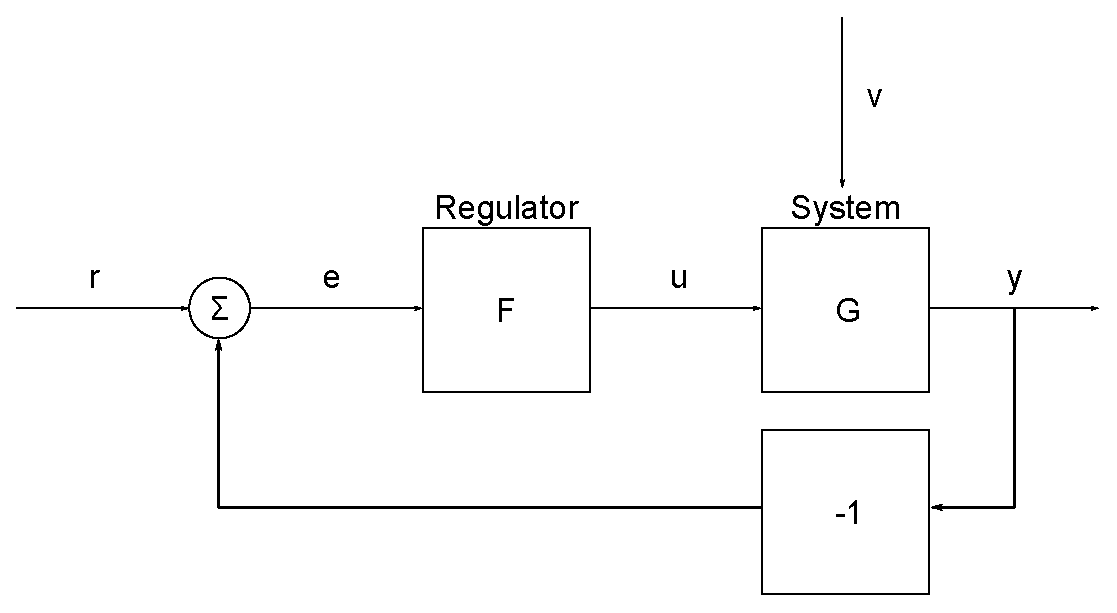
\includegraphics[width = \textwidth]{./Images/negative_feedback.eps}
	\caption{Schematisk illustration av ett enkelt negativt återkopplad system.}
	\label{fig:negative_feedback}
\end{figure}

\paragraph{Beskrivning av systemet}
Vi börjar beskrivningen av systemet med att inte betrakta störningar. I ena ändpunkten har vi
\begin{align*}
	Y = GU = GFE.
\end{align*}
Summationskomponenten till vänster ger oss
\begin{align*}
	E = R - Y,
\end{align*}
och därmed
\begin{align*}
	Y = GFR - GFY.
\end{align*}
Därmed kan vi skriva
\begin{align*}
	Y = \frac{GF}{1 + GF}R.
\end{align*}

\paragraph{Återkopplad överföringsfunktion}
För ett återkopplad system som kan skrivas som $Y = G_{\text{C}}R$ definieras $G_{\text{C}}$ som den återkopplade överföringsfunktionen. För systemet ovan har vi alltså
\begin{align*}
	G_{\text{C}} = \frac{GF}{1 + GF}R.
\end{align*}

\paragraph{Samband mellan reglerfel och referens}
Alternativt kan vi lösa systemet ovan för att få
\begin{align*}
	R - E = GFE,\ E = \frac{1}{1 + GF}R.
\end{align*}

\paragraph{Samband mellan referens och insignal}
Systemet ovan kan även lösas för att ge
\begin{align*}
	U = FR - FY = FR - GFU,\ U = \frac{F}{1  + GF}R.
\end{align*}

\paragraph{Slutna systems poler}
Vi ser att slutna system har poler där $1 + GF = 0$. Därmed bestäms systemets stabilitet av systemet och regulatorn.

\paragraph{P-reglering}
Principet i P-reglering är att välja en styrsignal som är proportionell mot storleken av felet, alltså
\begin{align*}
	u = K(r - y) = Ke.
\end{align*}
Det är här klart att för att få negativ återkoppling väljer vi $K > 0$.

Denna regleringsmetoden
\begin{itemize}
	\item minskar inverkan av störning och modellfel för ett bra val av $K$.
	\item ökar snabbheten vid insvängning.
	\item stabiliserar instabila system.
\end{itemize}
Däremot kan regleringen gå fel om t.ex.
\begin{itemize}
	\item systemet inte uppför sig som man tror.
	\item man har begränsningar i styrförmåga.
	\item man får instabilitet på grund av återkopplingen.
\end{itemize}

Det är även ett problem att om felet är stationärt, är även styrsignalen det, så även om du har ett nollskild fel klarar inte systemet nödvändigtvis anpassa sig.

\paragraph{PID-reglering}
PID står för proportionell integrerande deriverande. Denna sortens reglering löser många reglerproblem. Med PID-reglering väljer vi styrsignlaen
\begin{align*}
	u = K_{\text{P}}e + K_{\text{I}}\integ{t_{0}}{t}{\tau}{e} + K_{\text{D}}\dv{e}{t}.
\end{align*}
Alternativt kan vi skriva det som
\begin{align*}
	u = K\left(e + \frac{1}{T_{\text{I}}}\integ{t_{0}}{t}{\tau}{e} + T_{\text{D}}\dv{e}{t}\right).
\end{align*}

De tre ingående termerna i styrsignalen är
\begin{itemize}
	\item proportionell återkoppling, som betraktar det nuvarande felet.
	\item integrerande återkoppling, som betraktar hur felet har uppfört sig.
	\item deriverande återkoppling, som betraktar hur felet kommer att uppföra sig.
\end{itemize}

\paragraph{PI-reglering}
PI-reglering använder ej den deriverande återkopplingstermen. Vi ser härifrån att vid ett stationärt tillstånd är antingen $e = 0$, annars ökar eller minskar $u$ på grund av integraltermen.

Vi vill nu betrakta systemets insvängning. Om det stationära $\bar{u}$ krävs för att $e = 0$, har vi
\begin{align*}
	\bar{u} = K\left(e + \frac{1}{T_{\text{I}}}\integ{t_{0}}{t}{\tau}{e}\right).
\end{align*}
Vid att derivera detta fås
\begin{align*}
	K\left(\dv{e}{t} + \frac{1}{T_{\text{I}}}e\right) = 0,
\end{align*}
med lösning proportionell mot $e^{-\frac{t}{T_{\text{I}}}}$.

Notera att om man har stort fel kan PI-reglering ge problem. Därför använder man det typiskt när felen är små.

\paragraph{PI-reglering i Laplacevärlden}
Vid att Laplacetransformera uttrycket för styrsignalen i en PI-regulator, nämligen
\begin{align*}
	u = K\left(e + \frac{1}{T_{\text{I}}}\integ{t_{0}}{t}{\tau}{e}\right),
\end{align*}
fås
\begin{align*}
	U = K\left(E + \frac{1}{T_{\text{I}}s}E\right),
\end{align*}
och enligt figur \ref{fig:negative_feedback} ser vi att
\begin{align*}
	F(s) = K\left(1 + \frac{1}{T_{\text{I}}s}\right).
\end{align*}